% !TeX spellcheck = en_US
\documentclass{report}
\usepackage{paccosp}
	\makeindex
\begin{document}
	\title{Stochastic Processes notes}
	\author{Kotatsu}
	\date{\small vaffanculo}
	\maketitle
	\pagenumbering{Roman}
	\begin{preface}
Let's have a fucking party!
		
		\vskip1.2cm
		
		\hfill Kotatsu
	\end{preface}
	\clearpage
	\tableofcontents
	\pagenumbering{arabic}
\chapter{Brownian Motion}	
	\section{Continuity of stochastic processes}
	The sample path in a discrete scenario is given by
	\begin{equation*}
		\pr(X(t)<x|\F_{s})=\pr(X(t)<x|X_{s}).
	\end{equation*}
	This gives us a sample path like this:
	IMMAGINE
	We want to think, though, about a continuous space and time process: IMMAGINE
	How can we define the continuity of the sample paths? and how can we check this property? There are some possible definitions of continuity. To control for their robustness we check whether according to each of these definitions the Poisson process, a discrete process, is correctly classified as non continuous.
	\begin{definition}
		A stochastic process $\{M(t)\}$ is said to be a \emph{counting process} if:
		\begin{enumerate}[i.]
			\item $M(t)>0$;
			\item $M(t)$ is an integer;
			\item $M(t)$ is increasing, meaning that $s\leq t\implies M(s)\leq M(t)$.
		\end{enumerate}
	\end{definition}
	In general, these processes count how many times an event happens.
	\begin{definition}
		A Poisson process is a counting process such that:
		\begin{enumerate}
			\item $N(0)=0$;
			\item for $t_1<t_2<t_3<t_4$ we have
			\begin{equation*}
				N(t_2)-N(t_1)\independent N(t_4)-N(t_3)
			\end{equation*}
			meaning that the increments are independent;
			\item for $\every h>0$ and $t>\tau$ it holds:
			\begin{equation*}
				N(t)-N(\tau)\sim N(t+h)-N(\tau+h)
			\end{equation*}
			meaning that the increments are stationary (the origin start doesn't matter);
			\item we have $$\pr(N(t)=k)=\frac{(\lambda t)^{k}}{k!}e^{-\lambda t}\qquad\text{for } k=0,1,\ldots$$
		\end{enumerate}
	\end{definition}
	IMMAGINE\\
	The inter-arrival times are i.i.d. \rv s distributed as
	\begin{equation*}
		T_i\distexp{\lambda}.
	\end{equation*}
	The continuity of sample paths can be characterized in four different ways:
	\begin{enumerate}
		\item \emph{Continuity in mean squares}: we have this if for $\every t\geq0$ we have
		\begin{equation*}
			\lim_{s\to t}\ev\left[|X(t)-X(s)|^{2}\right]=0.
		\end{equation*}
		So according to this definition, the mean square of the distance goes to 0 if we go near $s$.
		\item \emph{Continuity in probability}: we have this if for $\every t\geq0$ and $\every\varepsilon>0$ we have
		\begin{equation*}
			\lim_{s\to t}\pr(|X(t)-X(s)|>\varepsilon)=0.
		\end{equation*}
		This should be enough for all finite distributions, right?\footnote{First, but not last, question without an answer.}
		\begin{theorem}
			Let $\{X(t)\}$ be a stochastic process such that $\ev[X^{2}(t)]<\infty$ for all $t$. Then it is continuous in mean squares\ifonly{}:
			\begin{enumerate}
				\item $m(t)=\ev[X(t)]$ is continuous;
				\item the covariance function
				\begin{equation*}
					\Gamma(s,t)=\ev[(X(t)-m(t))(X(s)-m(s))]
				\end{equation*}
				is continuous on its diagonal set.
			\end{enumerate}
			\begin{fancyproof}
				Consider the expectation
				\begin{equation*}
					\ev\left[|X(t)-X(s)|^{2}\right]=\ev\left[|X^{2}(s)+X^{2}(t)-2X(t)X(s)|\right]\tag{\faAdjust}\label{boh}
				\end{equation*}
				but
				\begin{equation*}
					\ev\left[X^{2}(s)\right]=\ubracketthin{\ev\left[(X(s)-m(s))^{2}\right]}_{\Gamma(s,s)}+2m(s)\ev\left[X(s)\right]-m^{2}(s)
				\end{equation*}
				and
				\begin{equation*}
					\ev\left[X^{2}(t)\right]=\Gamma(t,t)+2m(t)\ev[X(t)]-m^{2}(t)
				\end{equation*}
				and, moreover,
				\begin{equation*}
					\ev[X(s)X(t)]=\Gamma(s,t)-\cancel{m(t)m(s)}+m(t)\ev[X(s)]+\cancel{m(s)\ev[X(t)]}.
				\end{equation*}
				So \ref{boh} becomes
				\begin{align*}
					\text{\faAdjust}&=\Gamma(s,s)+2m^{2}(s)-m^{2}(s)+\Gamma(t,t)+2m^{2}(t)-m^{2}(t)-2\ev\left[X(s)X(t)\right]\\
					&=\Gamma(s,s)+\Gamma(t,t)-2\Gamma(s,t)+m^{2}(t)+m^{2}(s)-2m(t)m(s)\\
					&=\Gamma(s,s)+\Gamma(t,t)-2\Gamma(s,t)+\left[m(t)-m(s)\right]^{2}.
				\end{align*}
				Hence, if $m(t)$ is continuous and $\Gamma(s,t)$ is continuous for $s=t$ then the process is continuous.
				\begin{equation*}
					\ev\left[|X(s)-X(t)|^{2}\right]\to0.
				\end{equation*}
				If this holds for $m(t)$ and $\Gamma(t,t)$
			\end{fancyproof}
		\end{theorem}
	\end{enumerate}
	\begin{figure}
		\centering
		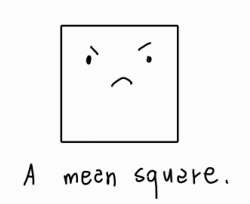
\includegraphics[width=0.5\linewidth]{img/screenshot001}
		\caption{Sei un fallito.}
		\label{fig:screenshot001}
	\end{figure}
	
\clearpage
\listoffigures  
\end{document} 


%THIS IS THE DARK AGE OF LOVE   